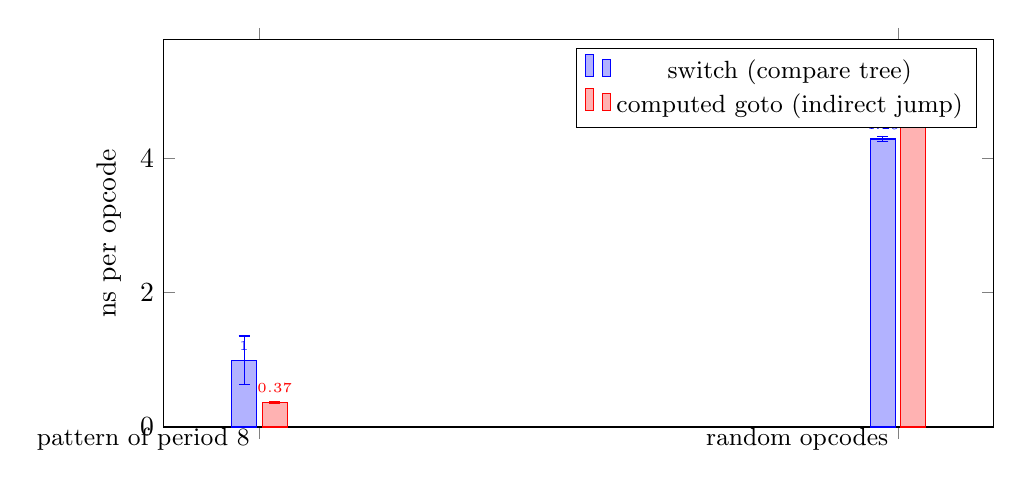
\begin{tikzpicture}
\begin{axis}[ybar, width=\textwidth, height=6.5cm, bar width=9pt, ymin=0, symbolic x coords={pattern of period 8,random opcodes}, xtick=data, x tick label style={rotate=0, anchor=east, font=\small}, ylabel={ns per opcode}, enlarge x limits=0.15, legend style={font=\small, at={(0.98,0.98)}, anchor=north east}, nodes near coords, nodes near coords style={font=\tiny}, every node near coord/.append style={/pgf/number format/.cd, fixed, precision=2}]
\addplot+[error bars/.cd, y dir=both, y explicit] coordinates {(pattern of period 8,0.9952) +- (0,0.3602) (random opcodes,4.2873) +- (0,0.0420)};
\addlegendentry{switch (compare tree)}
\addplot+[error bars/.cd, y dir=both, y explicit] coordinates {(pattern of period 8,0.3669) +- (0,0.0150) (random opcodes,5.2334) +- (0,0.0066)};
\addlegendentry{computed goto (indirect jump)}
\end{axis}
\end{tikzpicture}